\documentclass[aspectratio=169]{beamer} 
% no need of package graphicx in beamer

\title{CyberGoth Ballard}
\subtitle{A Platonic Reading of Crash}
\author{Verena Hermann} 
\date{}

\begin{document} 

\frame{\titlepage}     

\begin{frame}{The Republic}
	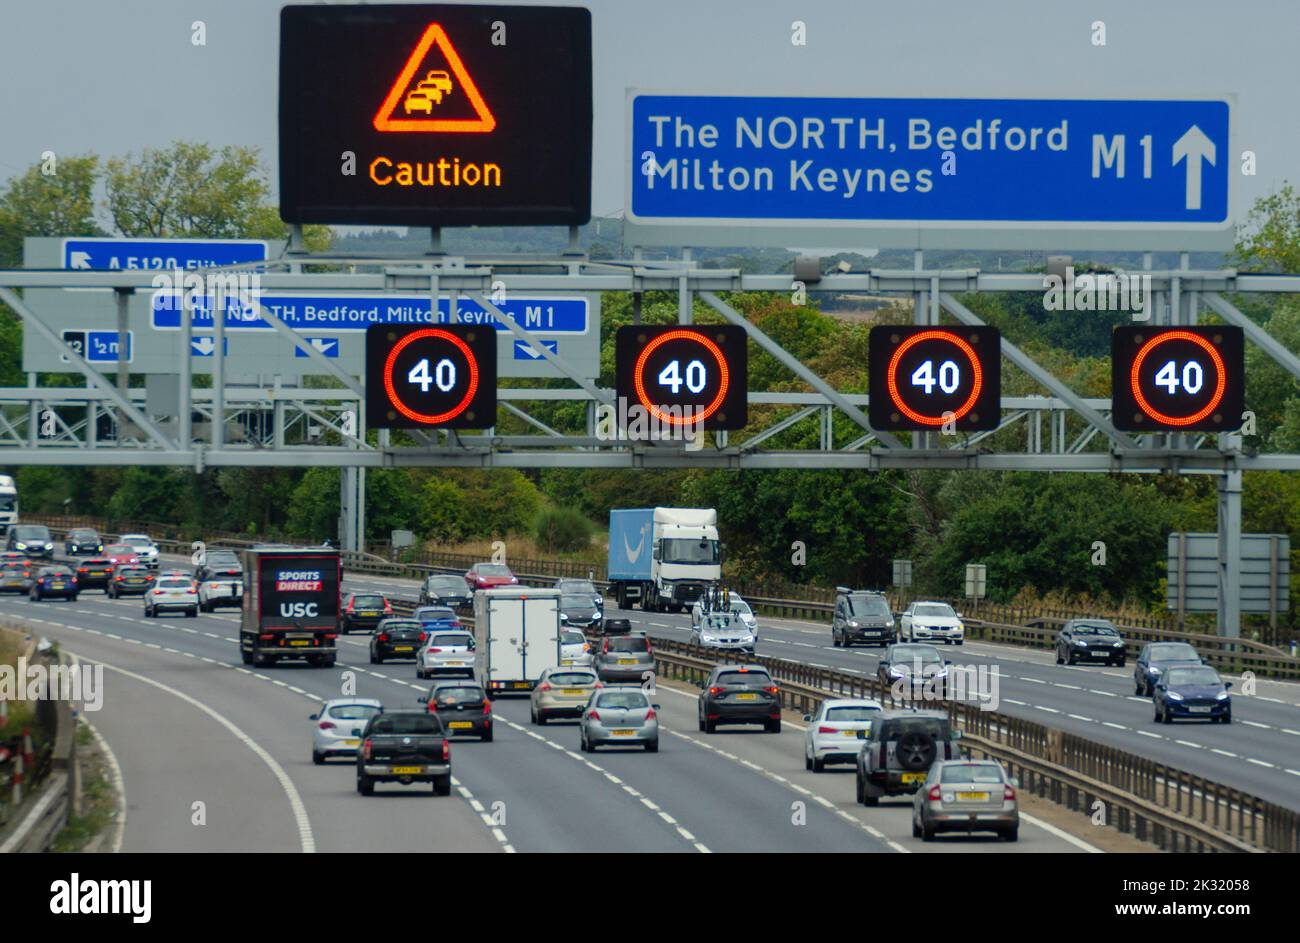
\includegraphics{illusions/motorway.jpg}
\end{frame} 

\begin{frame}{milieu of the cave}
\begin{figure}
   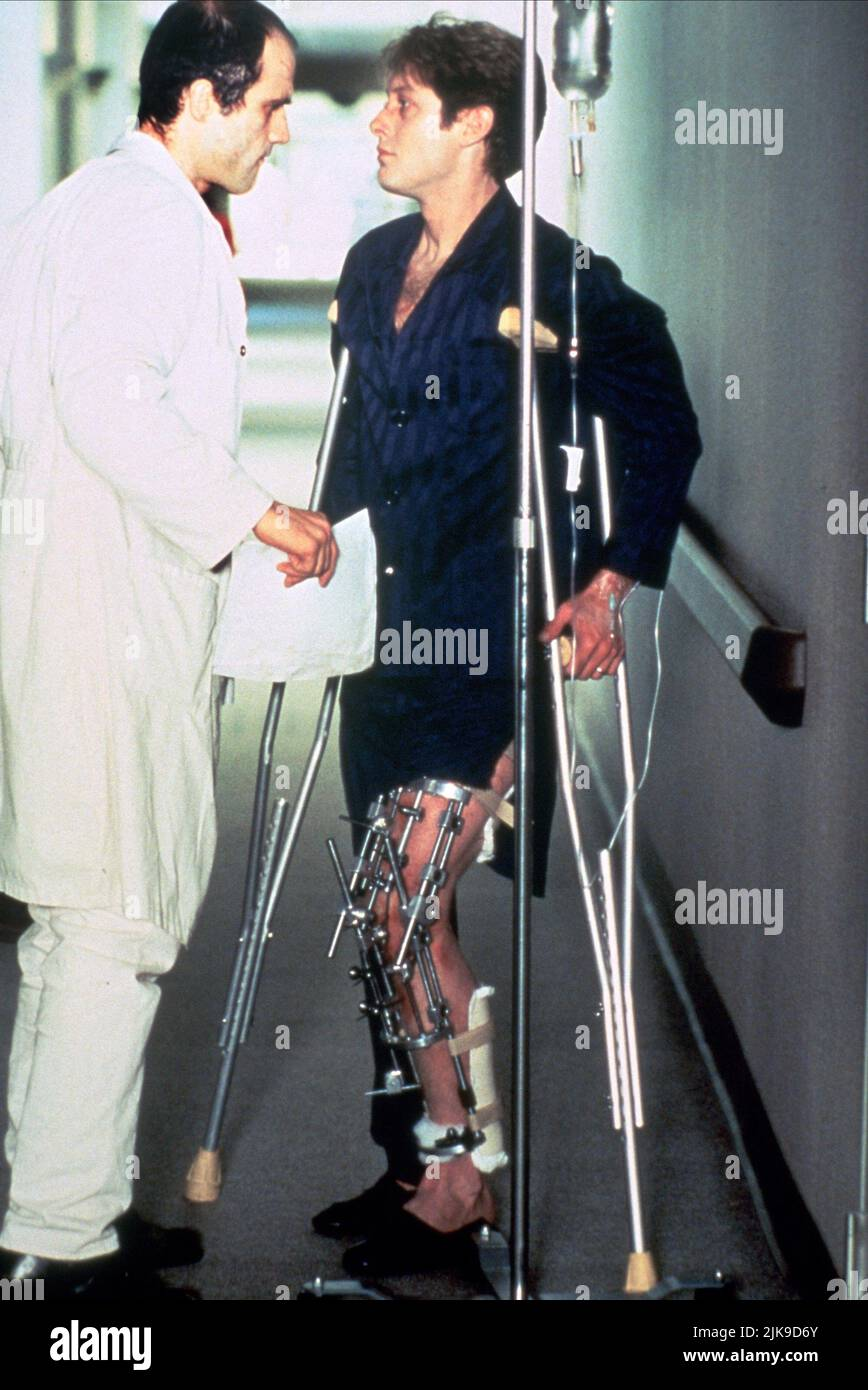
\includegraphics[scale=0.5]{illusions/drgood.jpg}
\end{figure}
"This sense of disembodiement, of the unreality of my own muscles and bones, increased when Vaughan appeared." (Ballard, 2014, 98)
\end{frame} 

\begin{frame}{Dianoia B} 
	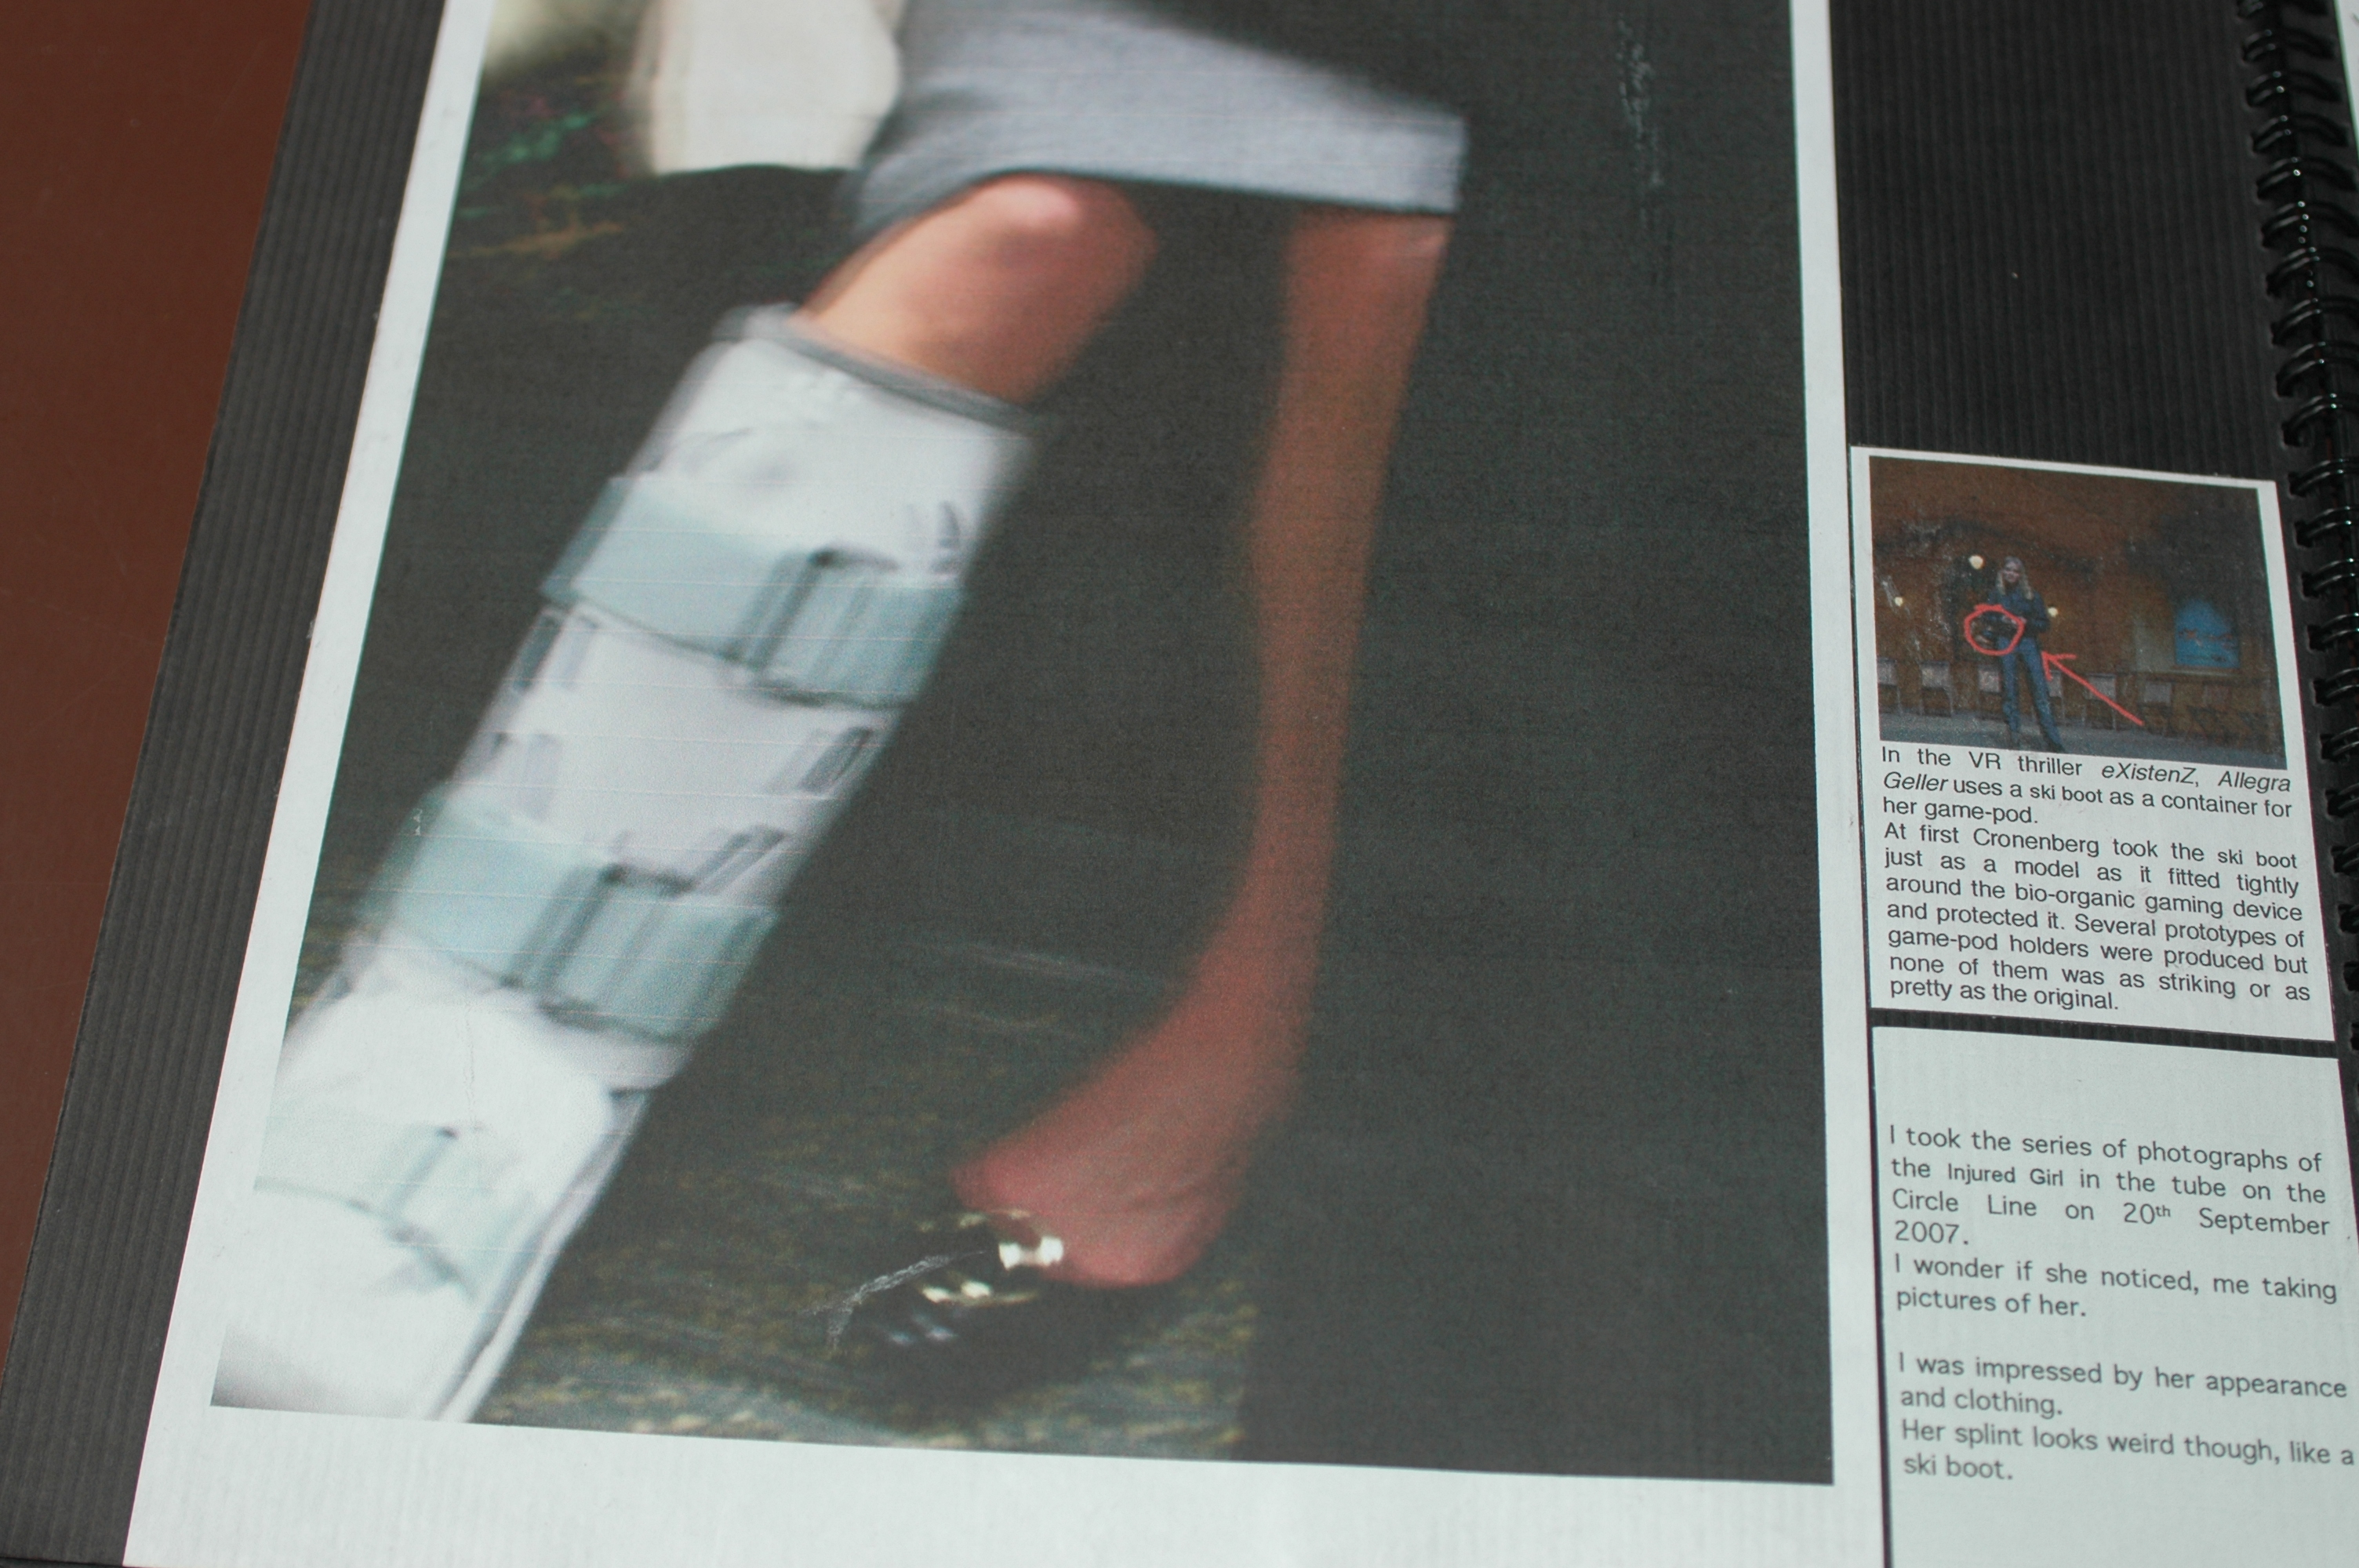
\includegraphics[scale=0.47]{illusions/injured_girl01.jpg}
\end{frame} 

\begin{frame}{Form in CyberGothic} 
	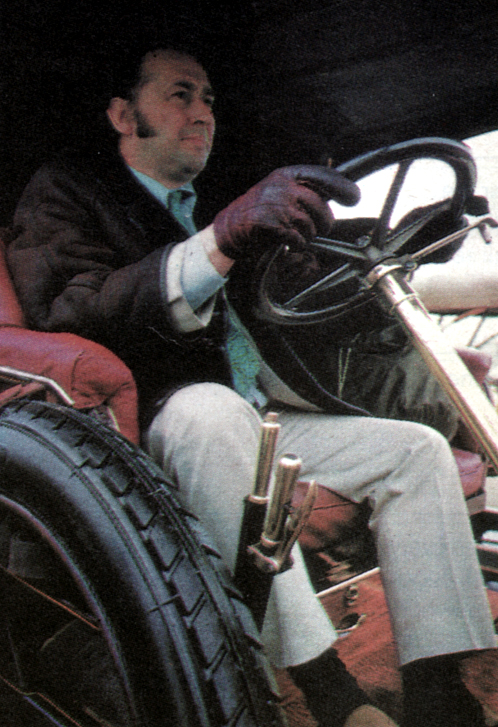
\includegraphics[scale=0.3]{illusions/JGB_at_wheel_drivemag-1580899123.jpg}
	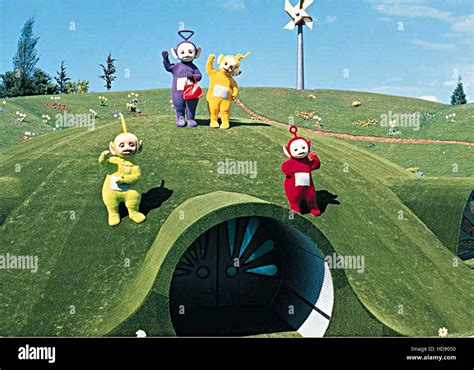
\includegraphics[scale=0.5]{illusions/teletubbies.jpg}
\end{frame}

\begin{frame}{conclusion /Smiley of the Sun} 
	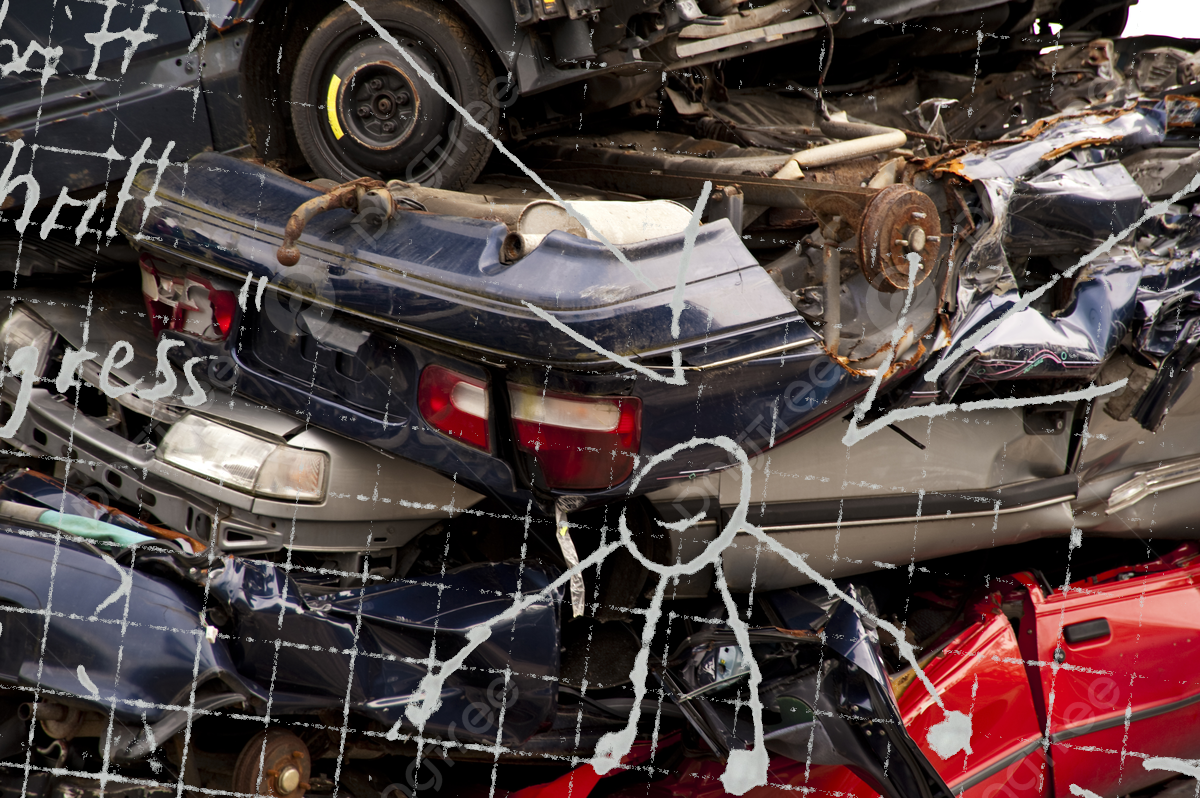
\includegraphics{illusions/peras01.png}
\end{frame}

\end{document}
